	%import packages%
\documentclass[12pt]{report}
\usepackage[a4paper]{geometry}
\usepackage[myheadings]{fullpage}
\usepackage{fancyhdr}
\usepackage{lastpage}
\usepackage{graphicx, wrapfig, subcaption, setspace, booktabs}
\usepackage[T1]{fontenc}
\usepackage[font=small, labelfont=bf]{caption}
\usepackage{fourier}
\usepackage[protrusion=true, expansion=true]{microtype}
\usepackage[francais]{babel}
\usepackage{sectsty}
\usepackage{url, lipsum}
\usepackage{tgbonum}
\usepackage{hyperref}
\usepackage{xcolor}
\usepackage{graphicx}

\newcommand{\HRule}[1]{\rule{\linewidth}{#1}}
\onehalfspacing
\setcounter{tocdepth}{5}
\setcounter{secnumdepth}{5}


	%page de couverture%
\begin{document}
\begin{figure}[t]
	\includegraphics{./images/logo_esiee.jpeg/}
\end{figure}
{\fontfamily{cmr}\selectfont
\title{ \normalsize \textsc{}
	\\ [2.0cm]
	\HRule{0.5pt} \\
	\LARGE \textbf{\uppercase{Rapport de projet}
	\HRule{2pt} \\ [0.5cm]
	\normalsize \today \vspace*{5\baselineskip}}
	}

\date{25 juin 2019}

\author{
	Laurent DELATTE, Théo PERESSE-GOURBIL, Manon HERMANN \\ 
	ESIEE Paris \\
	Projet de traitement de données médicales }

\maketitle
\tableofcontents
\newpage


	%page de sommaire%
\sectionfont{\scshape}


	%pages de texte%
\section{Introduction}
	\subsection{Presentation générale}
Dans le cadre des ateliers de fin d'année de E1. Nous avons choisi le sujet "traitement de données médicales", groupe capteur. \\
Nous avons pour but de conceptualiser un outil d'aide au suivi médical e-santé. Et implémenter une solution, avec un prototype opérationnel sur les variations et les pathologies du rythme cardiaque.\\
L'objectif de ce projet est d'aider le professionnel médical à détecter une bradycardie, une tachycardie ou une irrégularité du rythme cardiaque, en fonction des résultats de la mesures cliniques du pouls. 

	\subsection{Problematique}
Nous avons choisi l'étude de ...

	\subsection{Objectif}
Réccupérer les mesures cliniques enregistrées sur une plateforme-forme e-santé via un web-service. Développer une mini-application web qui traite les données récupérées et ache les résultats en vue d'une aide au diagnostic.


\newpage

\section{Demarche Scientifique}
\begin{enumerate}


\end{enumerate}

\newpage

\section{Resultat obtenu}
	\subsection{Solution proposé}
Afin de répondre au mieux à la problématique, nous avons divisé le traitement en 3 fichiers :
\begin{itemize}
\item \textbf{index.html} qui est la page d'identification pour accéder à la base de données ;
\item \textbf{liste.php} qui est la page allant chercher les différentes sessions enregistrées sur la base ;
\item \textbf{donnees.php} qui contient l'algorithme pour afficher les résultats de l'analyse.
\end{itemize}

	\subsection{Réalisation}
Le premier fichier, composé de la page d'identification comprend un formulaire web qui demande un utilisateur et un mot de passe. Grace aux types \textit{input}, nous avons pu cacher les mots de passe et les rendre obligatoires.
Ce formulaire adresse ensuite 3 données à un script php : L'utilisateur, \textbf{jekill}, le mot de passe,\textbf{congrat\_10}, ainsi qu'un paramètre caché correspondant aux données pour récupérer la liste des sessions.
\\
Ce script php affiche par la suite la liste des sessions sous forme d'un formulaire html déroulant.
Cette fois-ci, on inverse les données, on ne demande que le numéro de session, l'utilisateur et le mot de passe sont passés en paramètres cachés.
Ces informations sont envoyées au web-service qui nous revoie un tableau comprenant toutes les informations de la base de donnée concernant le patient.
\\

Ce tableau est au format JSON. On doit alors décoder ce tableau avec la fonction \textit{json\_decode()}, qui permet au tableau d'être plus lisible. Une fois décodé, ce tableau est composé de 3 sous tableaux, que l'on scinde dans des variables séparées. Le premier tableau est traité simplement en affichant les informations qu'il contient. Nous avons aussi fait un traitement de ces informations afin de les afficher d'une certaine couleur en fonction du résultat des informations, afin qu'elle soit visible par un éventuel médecin. En effet, un sportif professionnel (ex session \textit{Alain Mimoun}, est normal qu'il ait un rythme cardiaque bas. Nous avons effectués ce traitement sur les sportifs, les fumeurs, ceux qui ont de la fièvre, ou les personnes en situation d'obésité. \\
Nous avons alors décidé de calculer certaines données, comme l'IMC, ou le positionnement dans la moyenne.
\newpage

Par la suite, nous avons traité les mesures afin de recalculer la moyenne, l'écart type ainsi que le min ou le max de chaque données, à savoir les BPM, le SPO2, la température et la date et l'heure à laquelle la mesure a été effectuée.
Le but de ce traitement était de retirer les mesures erronées qui faisait chuter ou augmenter les statistiques (ex : SPO2 à 0 car le doigt a été mal positionnée).
\\

Une fois ce traitement effectué, on créés un tableau récapitulatif avec les données qui ont été recalculées.
On passe alors les données dans l'arbre de décision affiché au-dessus. Cela nous permet d'afficher un résultat personnalisé en fonction des résultats de l'algorithme.
Cela nous donne alors le tableau suivant \textit{pour le patient n°19}:
\begin{figure}[h]
    \centerline{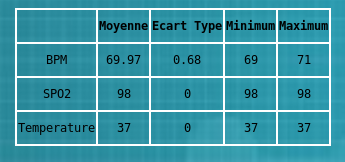
\includegraphics[width=10cm, height=5cm]{tableau.png}}
\end{figure}
\\
Par la suite, nous avons créé une graphique des BPM en fonction du temps. Cela a été possible grâce la librairie jp-graph. De plus, nous avons utilisé une fonction qui, à partir des tableaux traités, créer une image de ce graphique et le stock dans un dossier temporaire \textit{tmp}. Il nous suffit alors d'afficher cette image dans une balise html \textbf{<img .../>}. Par la suite, nous nous sommes aperçus que cette fonction ne marchait que sur un serveur sur les 2. Nous avons dû utiliser une variable du tableau \textbf{\$\_SERVER["HTTP\_HOST"]}, afin de savoir sur quel serveur est lancé le script. S’il s'agit du 147.215.191.33, on affiche le graphique, sinon on ne fait rien.
\\
Pour finir, nous avons fait différents fichiers CSS afin de mettre en forme de façon plus attirant les résultats que nous voulions afficher.
\\
Afin d'avoir un résultat plus "professionnel", nous avons décidés d'écrire des logs afin de garder en mémoire les actions qui ont été effectuées. On a donc créer une fonction qui prend en paramètre une string ainsi qu'un chemin vers un fichier. Cette fonction permet d'ouvrir le fichier en écriture, écrit dans ce fichier les informations passées en paramètres (ou la dernière erreur générée par PHP) puis ferme le fichier pour éviter les fuites mémoires.
Par la suite, nous avons voulu sécuriser les mots de passes à l'aide de hash. Cependant, nous n'avons pas réussi. Pour une raison obscure, lorsque nous comparions les hash stockées en mémoire et ceux qui avaient créés à partir des informations rentrées dans les champs \textit{user} et \textit{password}, même s’ils étaient identiques, le script disaient qu'ils étaient différents.


    \subsection{Tests}
Nous avons testé notre programme sur l'ensemble des patients répertoriés dans la base de données et pour chacun d'eux nous avons obtenu des résultats cohérents. \\
Nous avons par la suite fait des mesures expérimentales en classe grâce au matériel disponible pour créer une base de donnée plus large. Notons que le capteur de température était mal calibré, par conséquent nos mesures étaient erronées d'environ 2 °C par rapport a la réalité.


	\subsection{Sources}
\textit{Nous avons essayer, dans le mesure du possible, de n'utiliser que des sites certifiées HON. Fondation à but non lucratif, HON offre aux utilisateurs d’Internet des informations de santé fiables, avec près de 8000 sites accrédités, selon le code de conduite pour les sites Internet médicaux et de santé (HONcode)}
\begin{itemize}
\item Tableau et autres documentations du trouble cardiaque :       \textcolor{blue}{\url{https://www.fedecardio.org/sites/default/files/2019-TROUBLE-DU-RYTHME-Web.pdf}}
\item Enquète Canadienne sur le rythme cradiaque au repos : \textcolor{blue}{\url{https://www150.statcan.gc.ca/n1/pub/82-626-x/2013001/t004-fra.htm}}
\item Mise en abyme des maladies cardio vasculaire : \textcolor{blue}{\url{https://www.passeportsante.net/fr/Maux/Problemes/Fiche.aspx?doc=arythmie_cardiaque_pm}}
\item Irregularite du rythme cradiaque (causes + conseils) : \textcolor{blue}{\url{https://www.medisite.fr/problemes-cardiovasculaires-definitions-rythme-cardiaque-vos-battements-de-coeur-sont-ils-reguliers.5493549.524154.html}}
\item Ressources pour les commandes php : \textcolor{blue}{\url{https://php.net/}}
\item Ressources pour les commandes html et css : \textcolor{blue}{\url{https://www.w3schools.com/}}
\item HONsearch : Recherchez uniquement sur des sites web médicaux fiables et dignes de confiance
\end{itemize}

\newpage

\section{Bilan Personnel}
\begin{enumerate}


\end{enumerate}

\newpage



\end{document}
